% 第2章
%!TEX root = main.tex

%%%%%%%%%%%%%%%%%%
\chapter{実験機体}
\label{aircraft}
%%%%%%%%%%%%%%%%%%

本章では,実験を行なった開発機体の開発コンセプトと,設計や搭載システムの概要を述べる.機体は,災害発生時,回転翼機モードで離陸し,上空で固定翼機モードへと遷移して被災地へ向かう.そして被災地上空へ到着した後,回転翼機モードへと遷移し,ホバリング飛行しながら,情報収集や着陸可能地点の検出を行なう.

\section{実験機の概要}
本研究グループの目的である,大規模災害発生時の任務遂行には,狭隘地への進入が必要な場合がある.また救援物資の運搬に利用する場合,救助者に近い距離で着陸を行なう可能性もあり,対人安全性の強化が必要である.さらに,空撮や着陸可能地点の検出には,安定した飛行とホバリングを行なう必要がある.

以上を踏まえて,機体製作にあたり以下の3点
	\begin{enumerate}
	\item 機体サイズの小型化
	\item 対人安全性を考慮
	\item ヘリコプタと同等のホバリング性能
	\end{enumerate}
をコンセプトとしている.2015年に,エアロセンス株式会社と共同開発を行なったが,本研究ではFig. \ref{fig:vtol23k}に示す後継機を用いている.

\hspace{5pt}

メインロータには,同軸二重反転ロータを使用する.二重反転ロータはシングルロータと比較して効率がよく,推力が大きいと言われている.また,ヘリコプタモード時に反トルクを打ち消すためのテールロータが不要になり,機体サイズの小型化を図れるという利点もある.この二重反転ロータユニットを胴体中央部に組み込むことで,ロータの機体外部への露出を防止し,対人安全性の強化を図っている.

\begin{figure}[H]
	\centering
	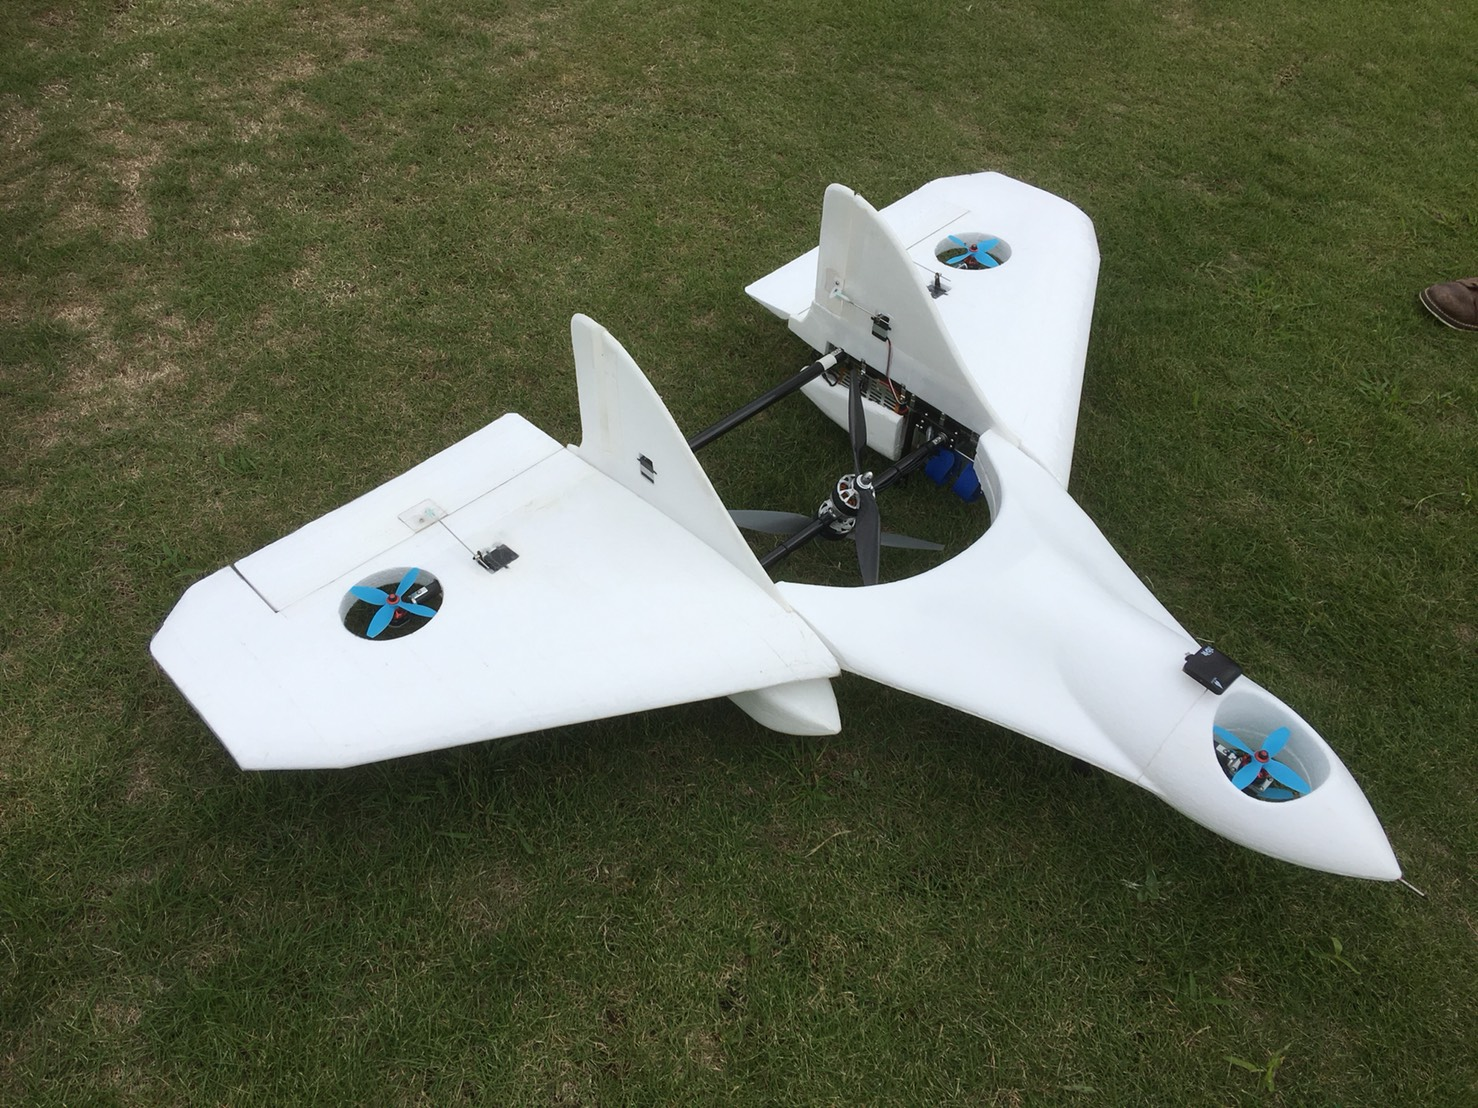
\includegraphics[clip,width=10.0cm,bb=0 0 1478 1108]{./z_figure_files/chapter2/1_vtol23K.JPG}
	\caption{Tilt rotor UAV}
	\label{fig:vtol23k}
\end{figure}

上下に取り付けられたメインロータは,それぞれ独立に駆動可能であるため,上下のロータで異なる回転数を実現できる.ホバリング時のヨー制御は,上下のロータの回転数を調整することで発生する反トルクの差を利用して行なう.メインロータを取り付けたティルト軸はサーボ機構を有しており,機体胴体に対してピッチ軸周りの回転自由度を有する.Fig. \ref{fig:tilt0} ~ \ref{fig:tilt90}に示すように,メインロータをティルトさせることで,ヘリコプタモード,遷移モード,飛行機モードの切り替えを行う.
\begin{figure}[h]
	\begin{center}
		\begin{tabular}{c}

			\begin{minipage}{0.33\hsize}
				\begin{center}
					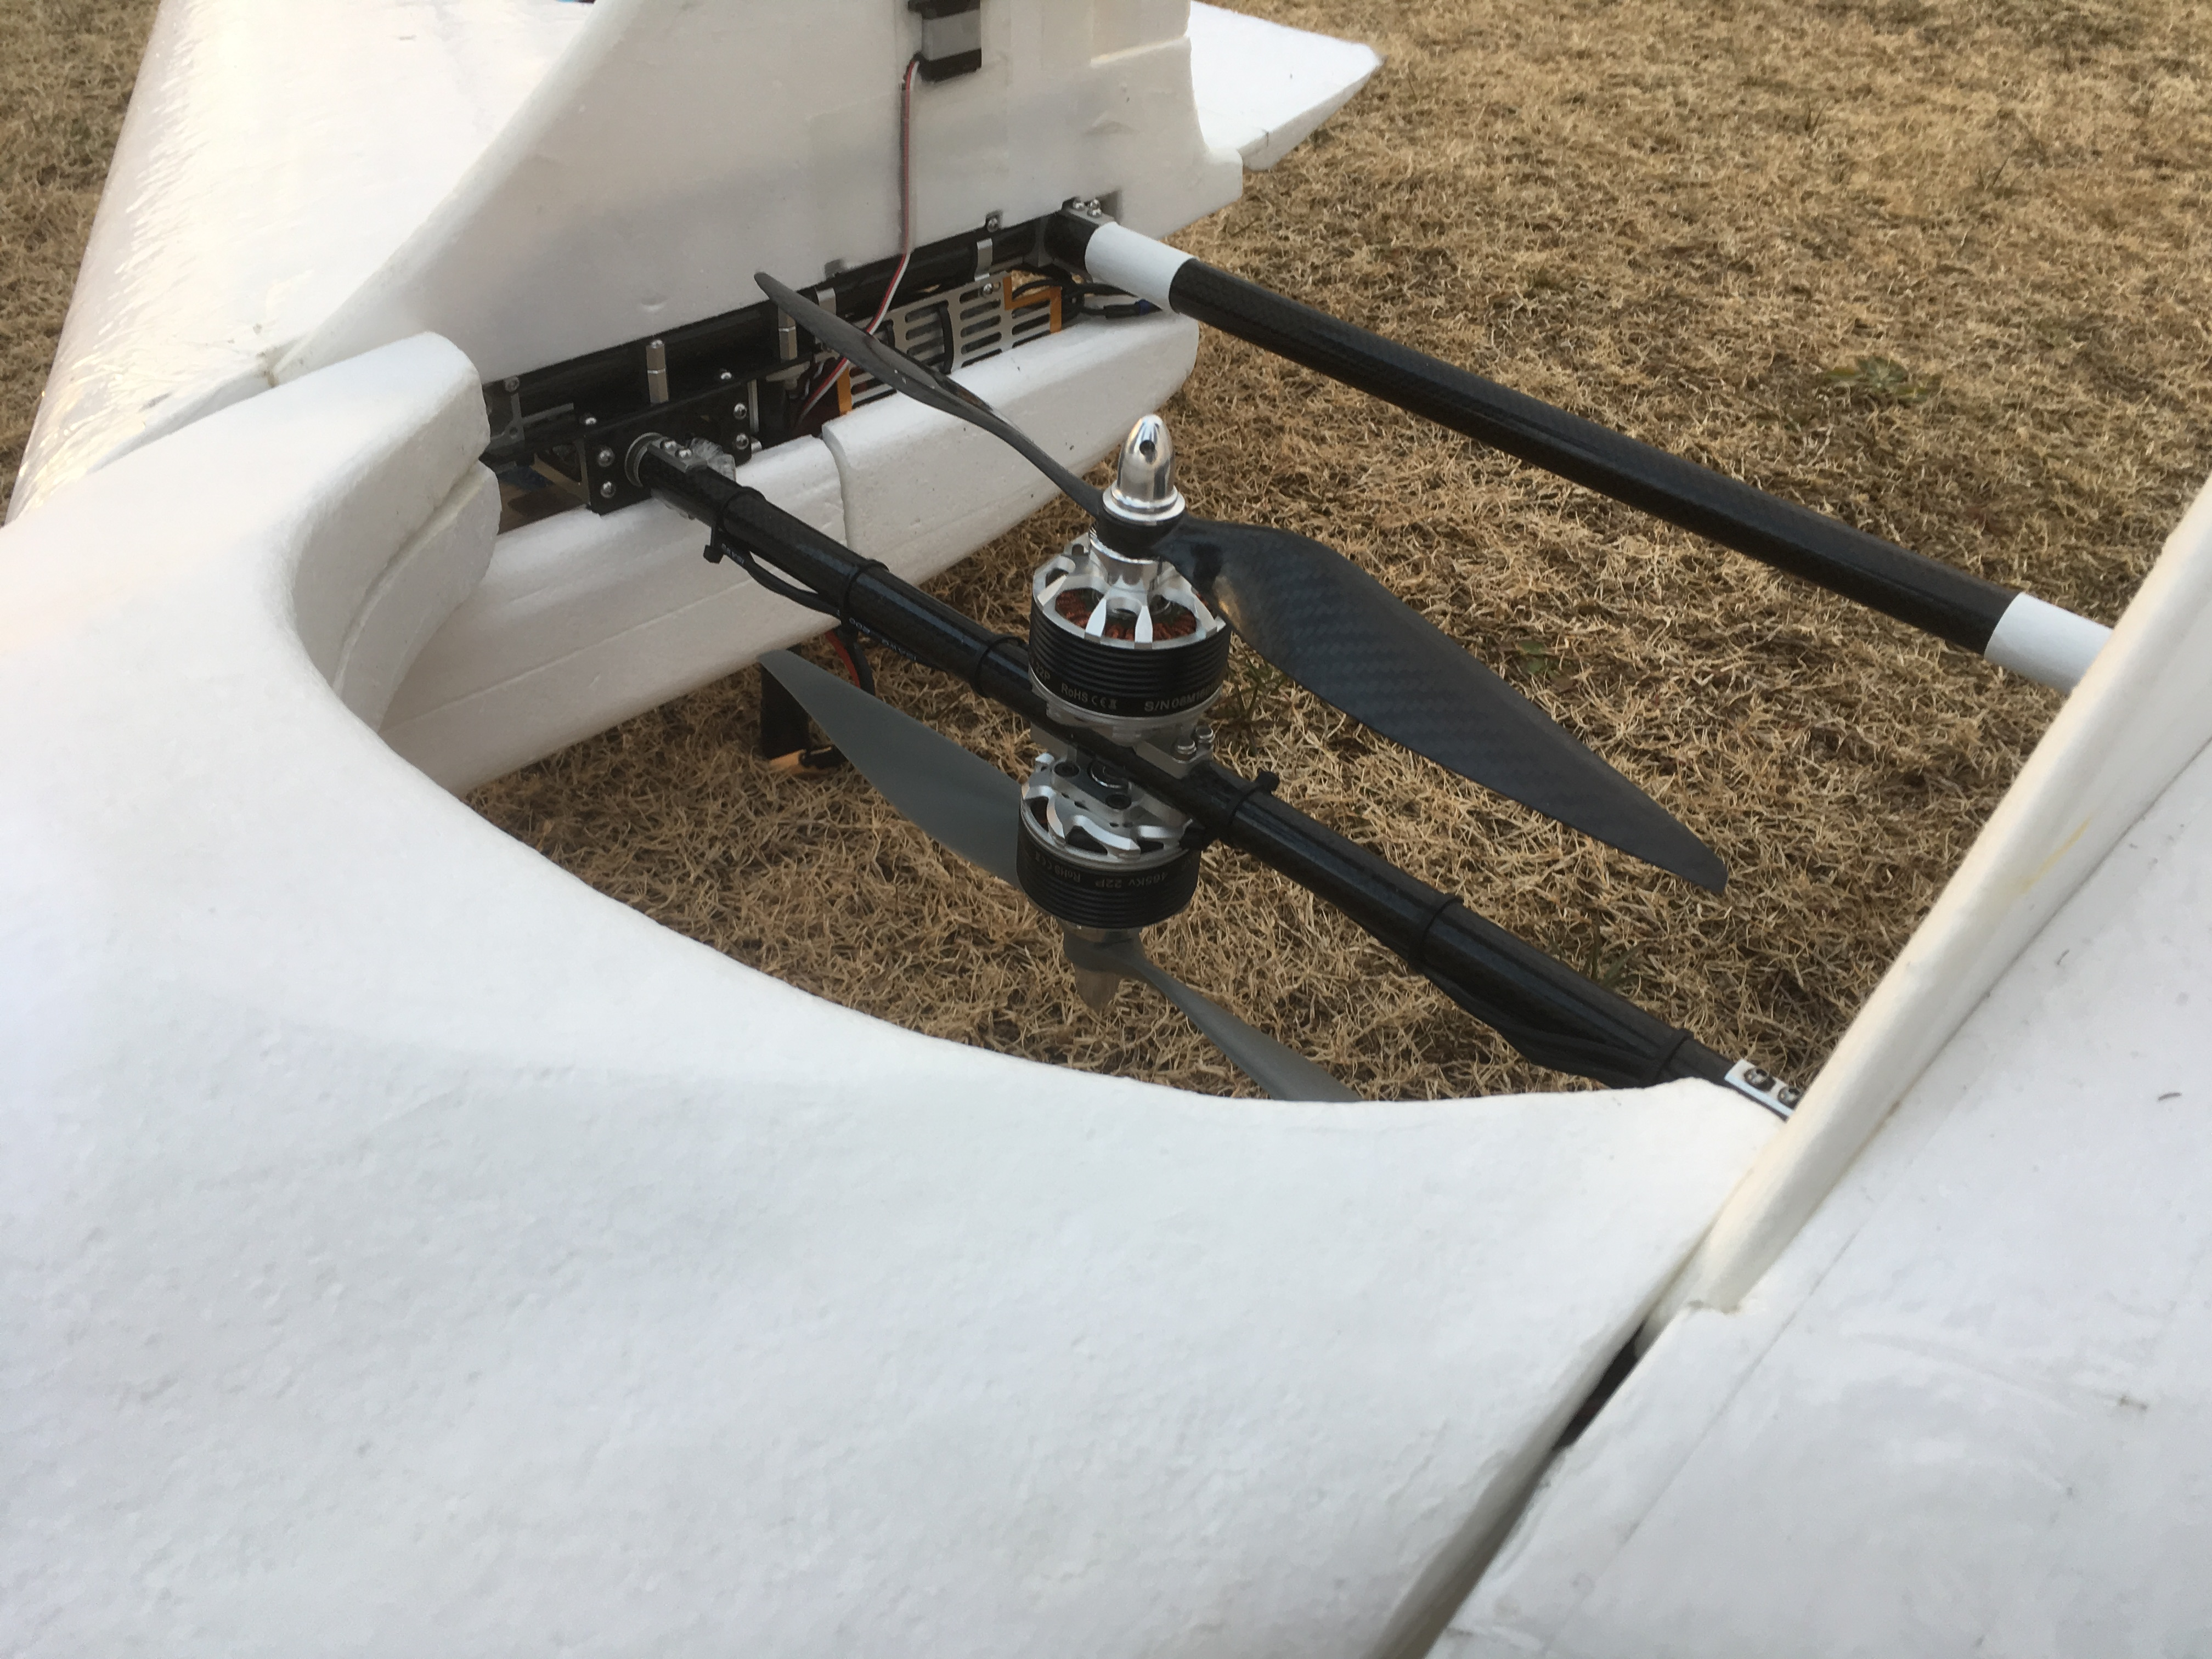
\includegraphics[clip,width=4.0cm,bb=0 0 4032 3024]{./z_figure_files/chapter2/2_tilt0.JPG}
					\caption{Helicopter Mode}
					\label{fig:tilt0}
				\end{center}
			\end{minipage}

			\begin{minipage}{0.33\hsize}
				\begin{center}
					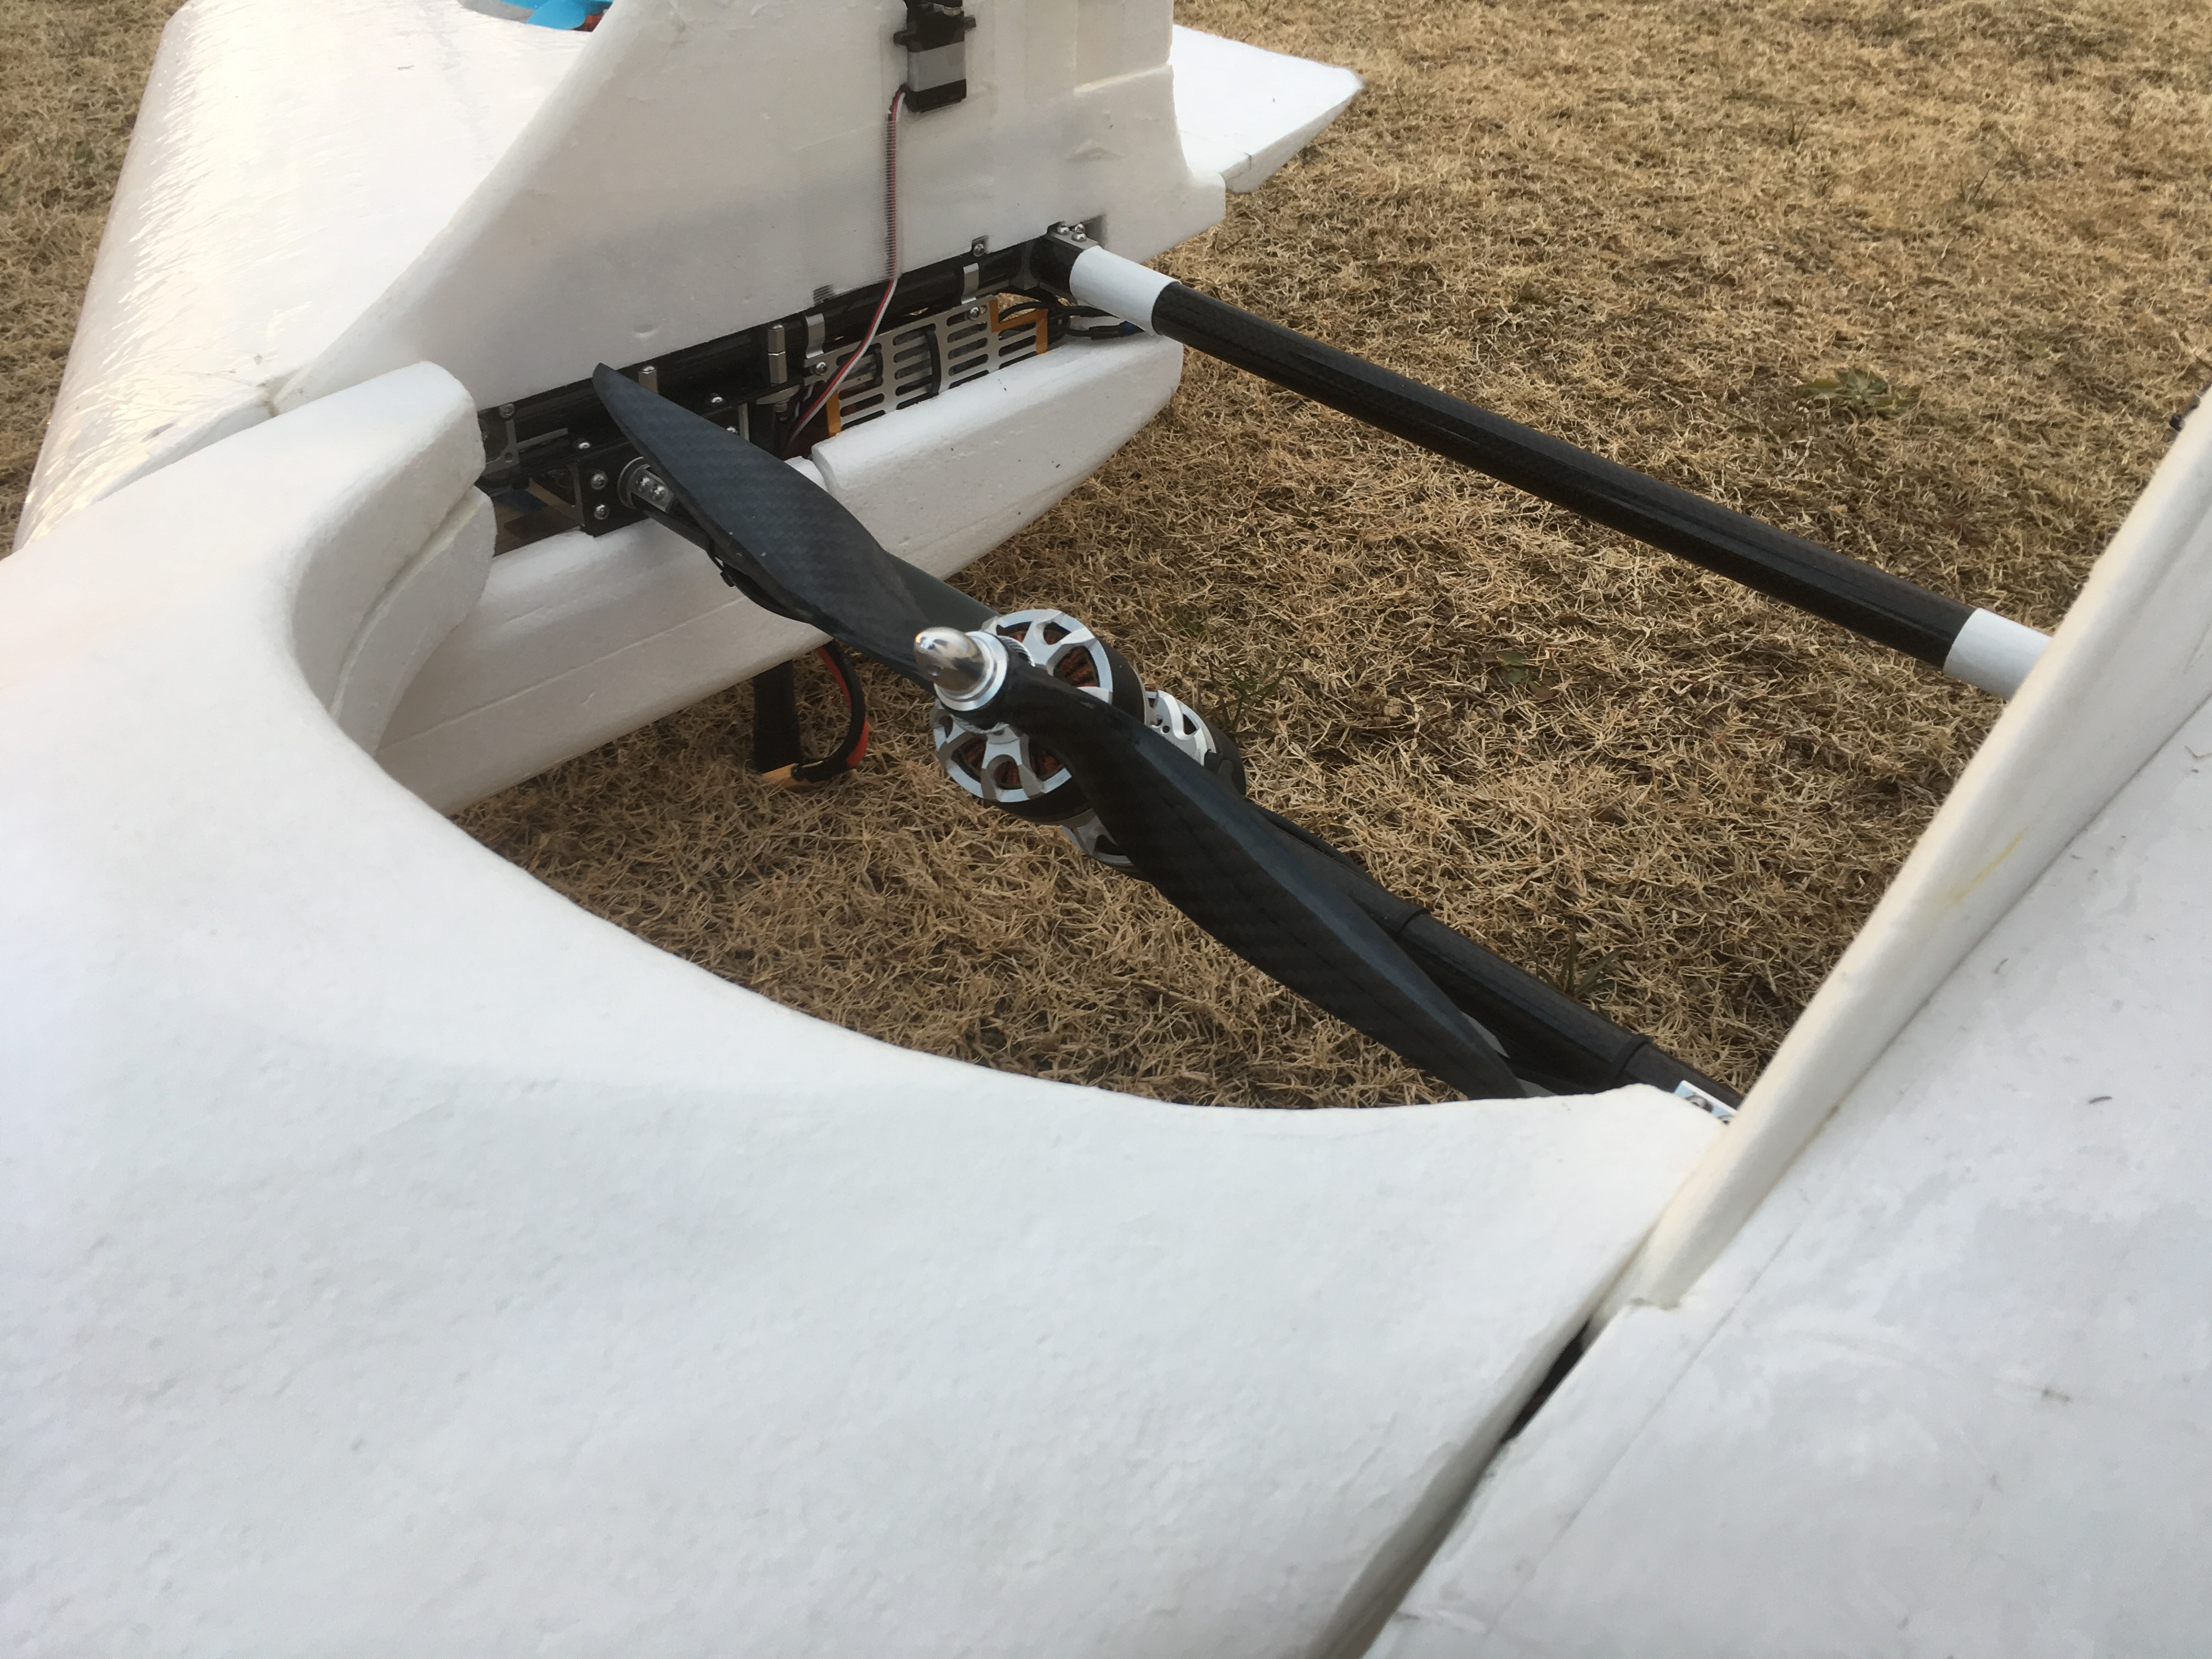
\includegraphics[clip,width=4.0cm,bb=0 0 4032 3024]{./z_figure_files/chapter2/3_tilt45.JPG}
					\caption{Transition Mode}
					\label{fig:tilt45}
				\end{center}
			\end{minipage}

			\begin{minipage}{0.33\hsize}
				\begin{center}
					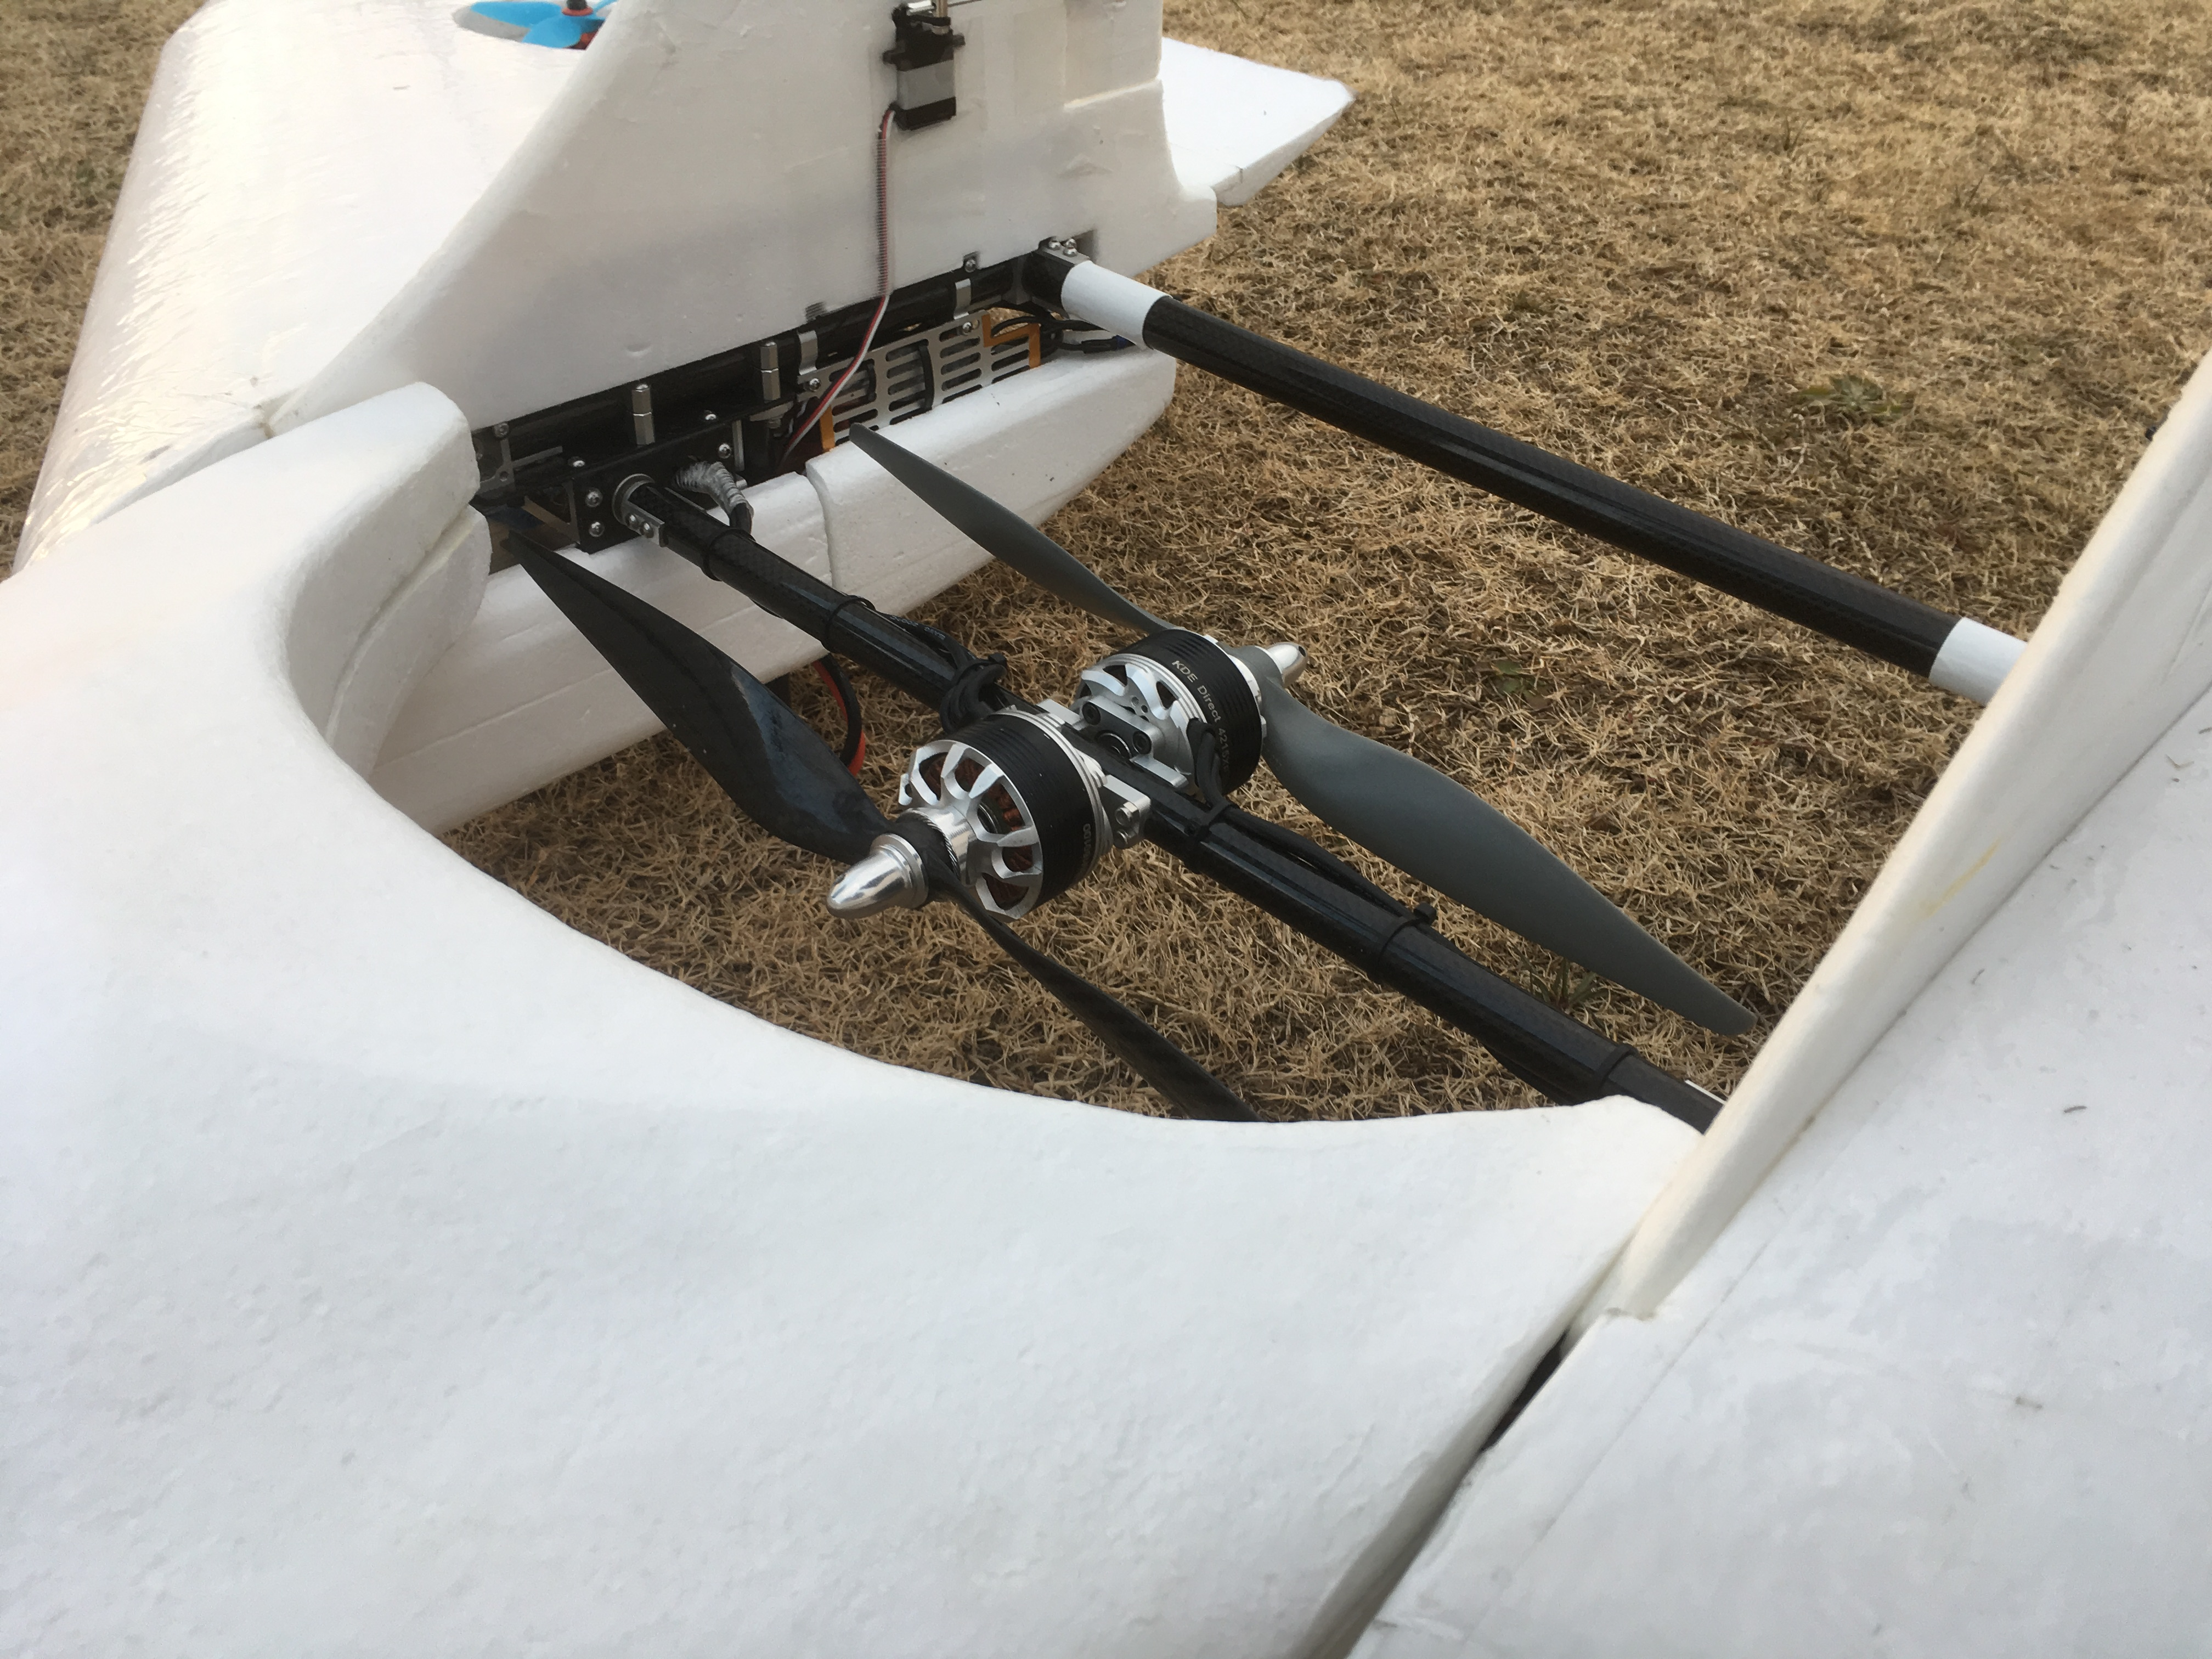
\includegraphics[clip,width=4.0cm,bb=0 0 4032 3024]{./z_figure_files/chapter2/4_tilt90.JPG}
					\caption{Airplane Mode}
					\label{fig:tilt90}
				\end{center}
			\end{minipage}

		\end{tabular}
	\end{center}
\end{figure}

 ヘリコプタモードにおいて,風などの外乱に対して安定したホバリングを行なうために,姿勢制御用のサブロータを左右翼端に1つずつ,機首部上下に2つ,計4つのサブロータを取り付けている(Fig. \ref{fig:sub1},~\ref{fig:sub2}).機首部のサブロータは二重反転ロータになっており,機首部のサブロータで発生する反トルクを打ち消すようになっている.ヘリコプタモードにおけるホバリング時には,サブロータとメインロータの出力やティルト角を調整し,機体重心周りのモーメントを発生させることでピッチ軸およびロール軸の制御を行なう.

\begin{figure}[h]
 \begin{center}
	 \begin{tabular}{c}

		 \begin{minipage}{0.49\hsize}
			 \begin{center}
				 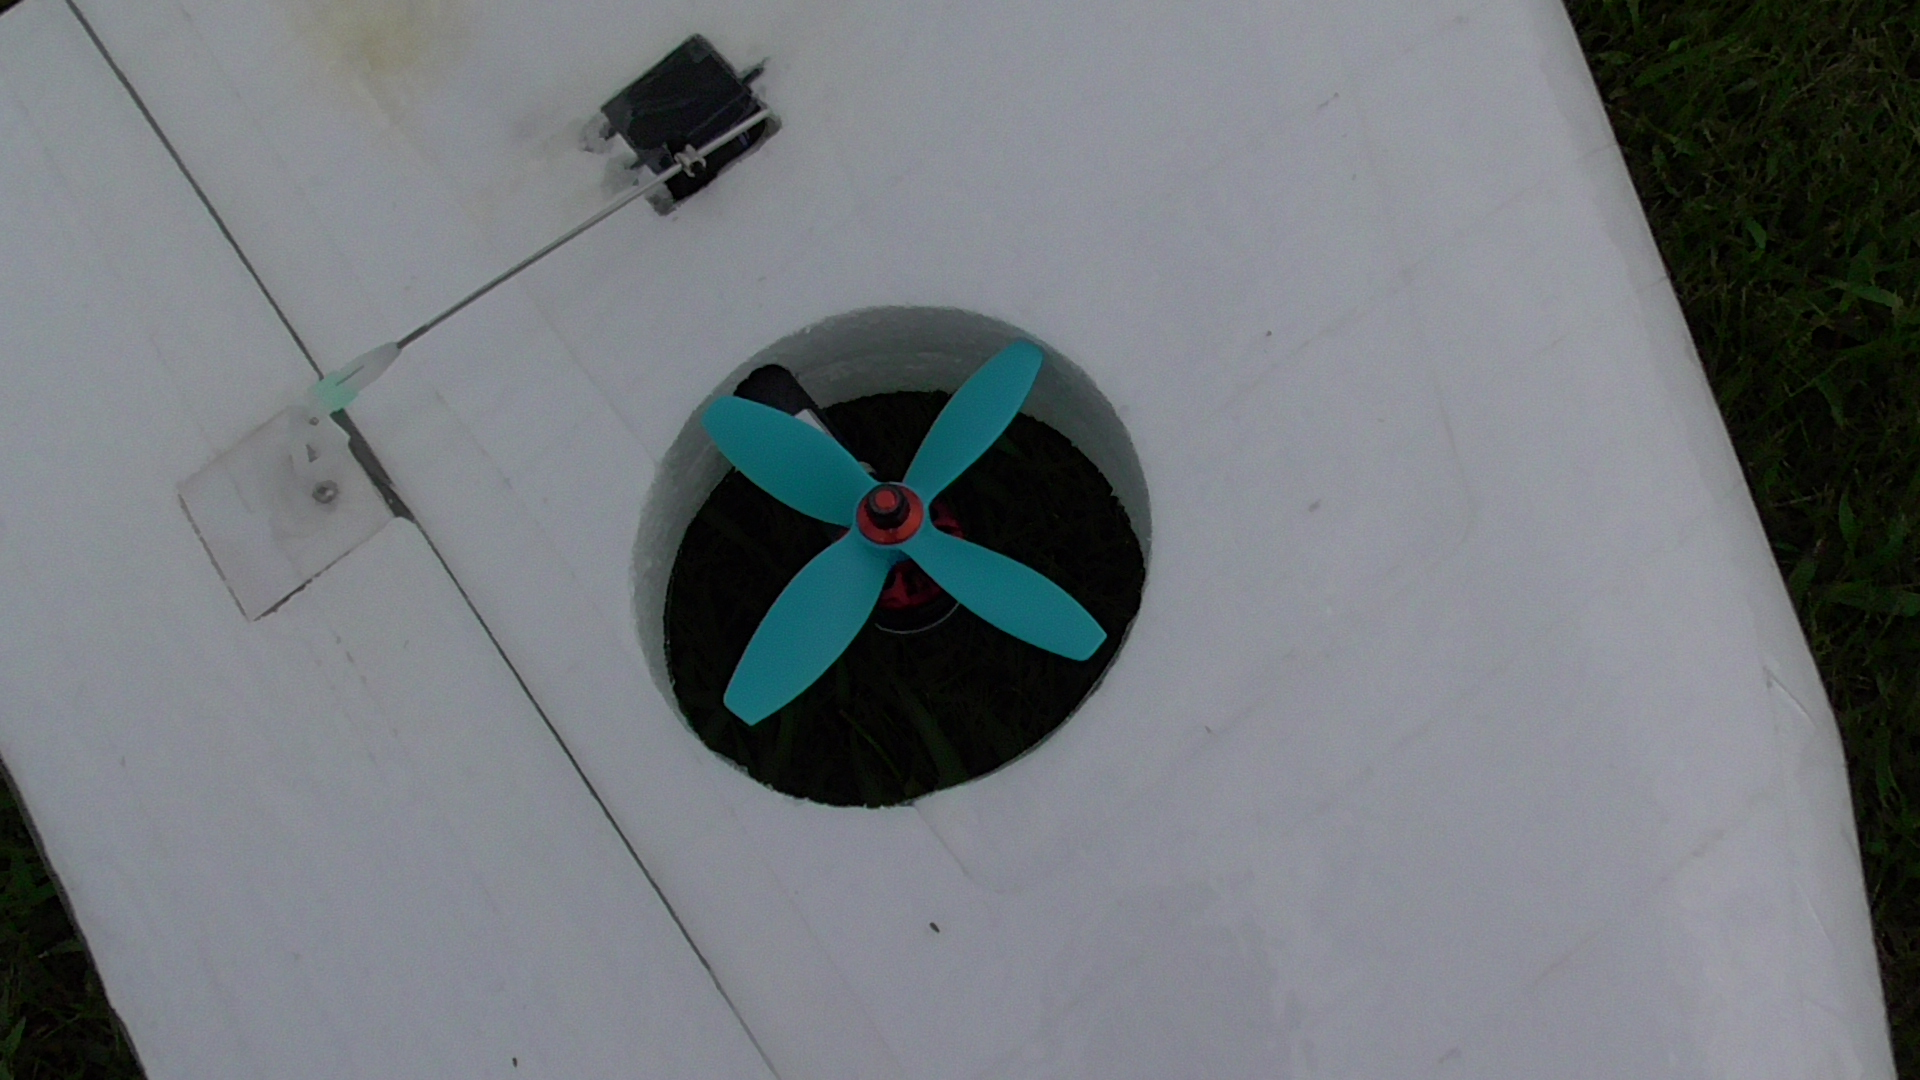
\includegraphics[clip,width=6.0cm,bb=0 0 1920 1080]{./z_figure_files/chapter2/5_Sub_rotor_wing.JPG}
				 \caption{Sub rotor (wing tip)}
				 \label{fig:sub1}
			 \end{center}
		 \end{minipage}

		 \begin{minipage}{0.49\hsize}
			 \begin{center}
				 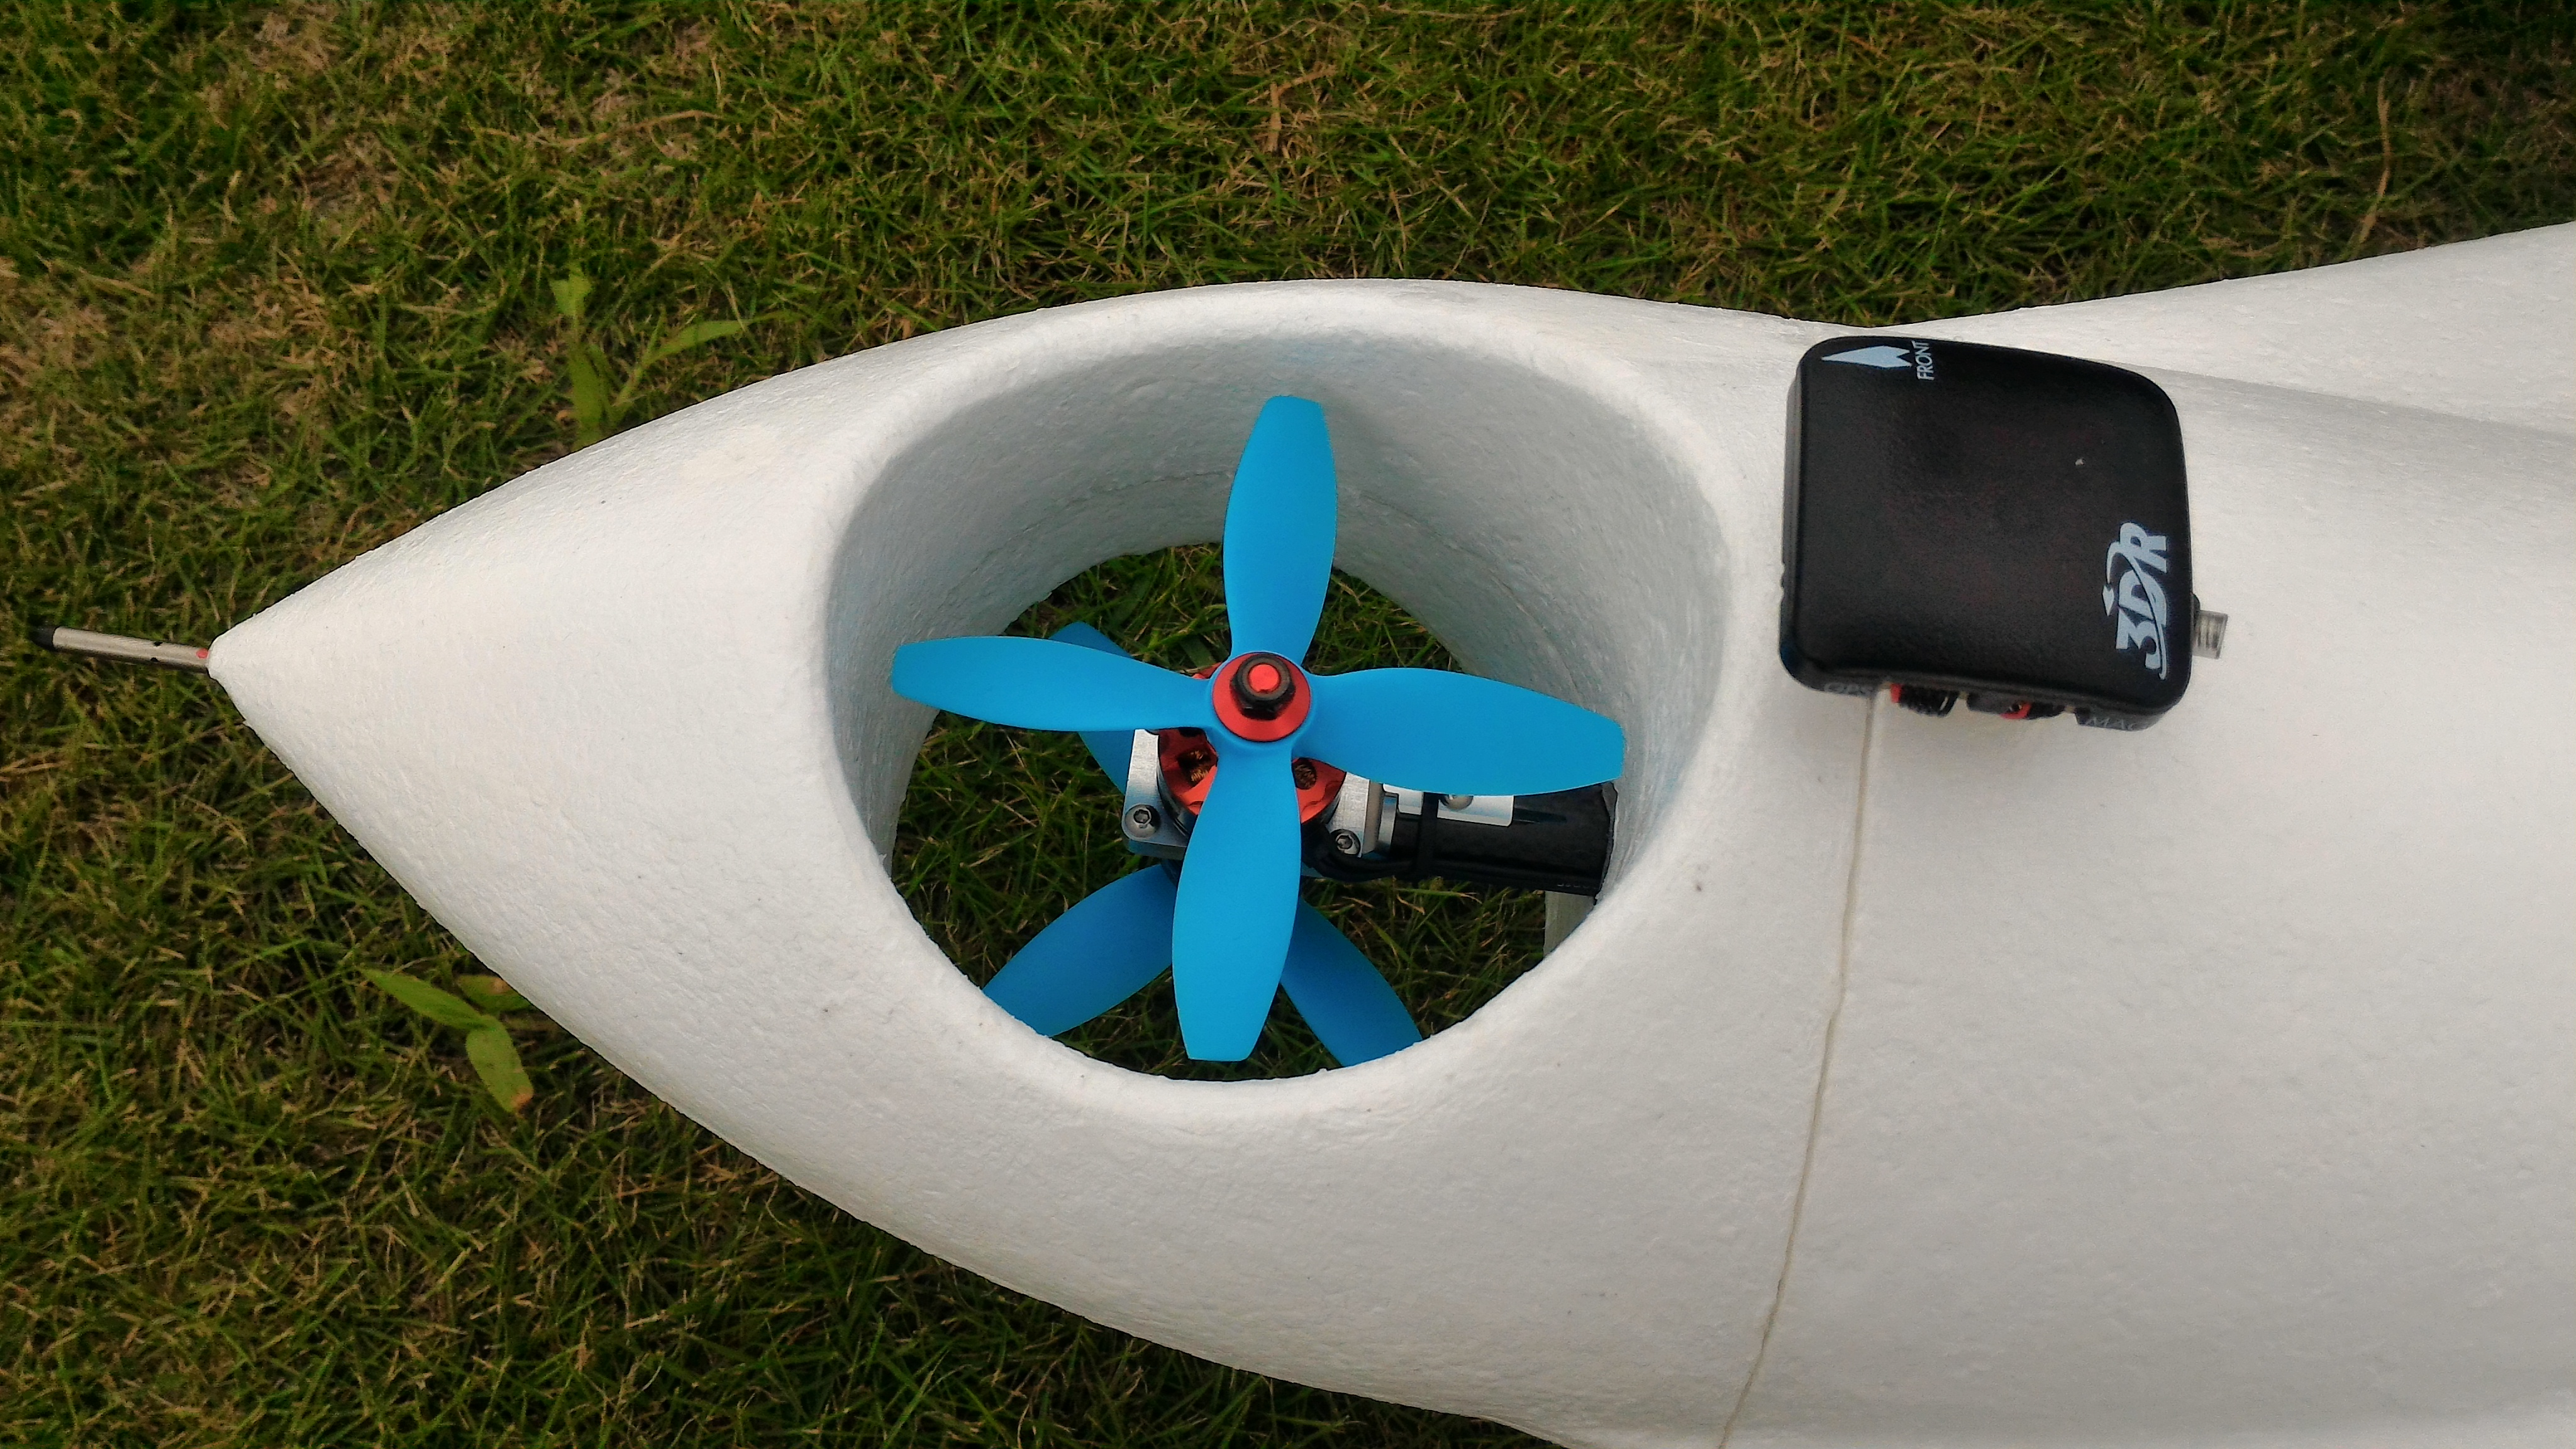
\includegraphics[clip,width=6.0cm,bb=0 0 4096 2304]{./z_figure_files/chapter2/6_Sub_rotor_nose.JPG}
				 \caption{Sub rotor (nose)}
				 \label{fig:sub2}
			 \end{center}
		 \end{minipage}

	 \end{tabular}
 \end{center}
\end{figure}

また,姿勢制御のための動翼として,左右で独立に動かすことができるエレボン(Fig. \ref{fig:elevon})が主翼後縁に取り付けられており,エルロンとしてのロール角制御と,エレベータとしてのピッチ角制御を行うことができる.また,垂直尾翼後縁には,ヨー角制御に用いるラダー(Fig. \ref{fig:rudder})が取り付けられている.\\

\begin{figure}[hb]
	\begin{center}
		\begin{tabular}{b}

			\begin{minipage}{0.49\hsize}
				\begin{center}
					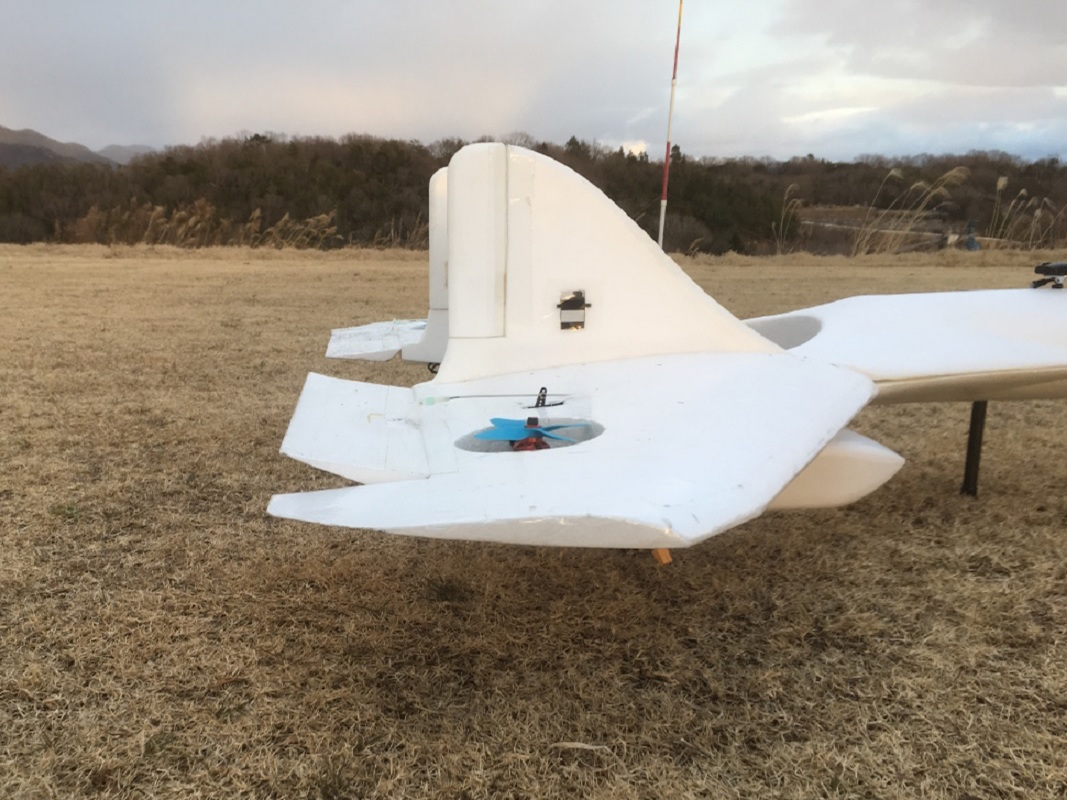
\includegraphics[clip,width=6.0cm,bb=0 0 1067 800]{./z_figure_files/chapter2/7_elevon.jpg}
					\caption{Elevon}
					\label{fig:elevon}
				\end{center}
			\end{minipage}

			\begin{minipage}{0.49\hsize}
				\begin{center}
					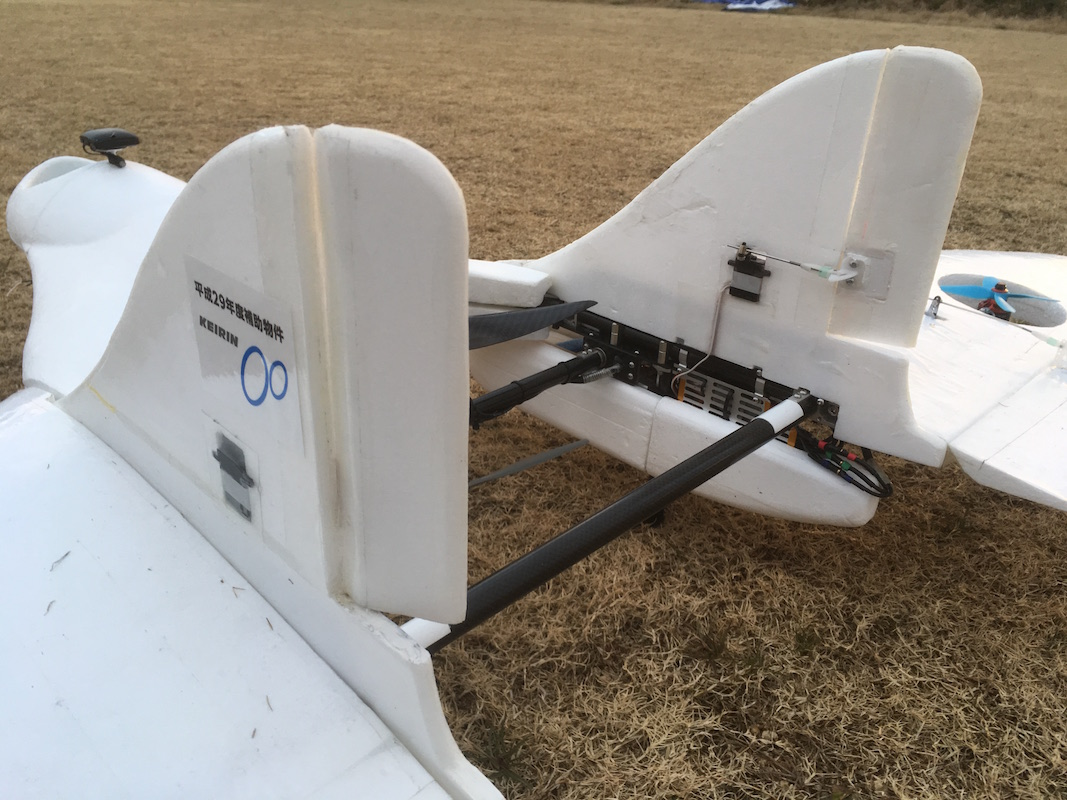
\includegraphics[clip,width=6.0cm,bb=0 0 1067 800]{./z_figure_files/chapter2/8_rudder.jpg}
					\caption{Rudder}
					\label{fig:rudder}
				\end{center}
			\end{minipage}

		\end{tabular}
	\end{center}
\end{figure}

Fig. \ref{fig:frame}は機体フレームである.フレームにはカーボンパイプを使用し,機体の軽量化を図りつつ剛性も確保している.また,Table \ref{spec}に機体サイズや機体を構成するハードウェア機器に関してまとめる.最後に,Fig. \ref{fig:wings},Table \ref{wingspec}に主翼と尾翼の面積や長さについてまとめる.面積や長さには,エレボンやラダーも含まれている.

%%%%%%%%%%%%%%%%%%%%%%
\section{搭載システム}
%%%%%%%%%%%%%%%%%%%%%%

正確な機体の運動制御のためには,機体の速度や姿勢などの飛行データを正確に得ることが必要である.本研究では,3軸加速度・角速度センサ,地磁気センサ,気圧センサを内蔵した小型の搭載コンピュータ(Fig. \ref{fig:pixhawk}),GPSセンサ(Fig. \ref{fig:GPS}),およびピトー管とよばれる対気速度計測装置(Fig. \ref{fig:pitot})を使用する.これらのセンサからの観測値をもとに,カルマンフィルタによって飛行状態が推定される.また,搭載コンピュータを用いて各ロータ推力などの制御量の計算を行なう.
\begin{table}[htb]
	\begin{center}
		\caption{Specifications of the tilt rotor UAV}
		\label{spec}
		\begin{tabular}{|c|c|}\hline
			Total length & 1.08[m] \\ \hline
			Total width & 1.43[m] \\ \hline
			Total weight & 5.738[kg]\\ \hline
			Main rotor motor & KDE4215XF-435 $\times$ 2\\ \hline
			Main propeller(upper) & MB-ARRIS-P1365C$13 \times 6.5$EP\\ \hline
			Main propeller(lower) & APC$13 \times 8.0$E\\ \hline
			Main rotor battery & 6S-6300mAh(30C)\\ \hline
			Main rotor maximum thrust(coaxial) & 6.209[kgf]\\ \hline
			Sub rotor motor & RM2204-2600 $\times$ 4\\ \hline
			Sub rotor propeller & Lumenier $4 \times 4 \times 4$\\ \hline
			Sub rotor and System battery & 4S-2200mAh(35C)\\ \hline
			Sub rotor maximum thrust(single) & 0.931[kgf]\\ \hline
		\end{tabular}
	\end{center}
\end{table}
\begin{figure}[hb]
	\begin{center}
		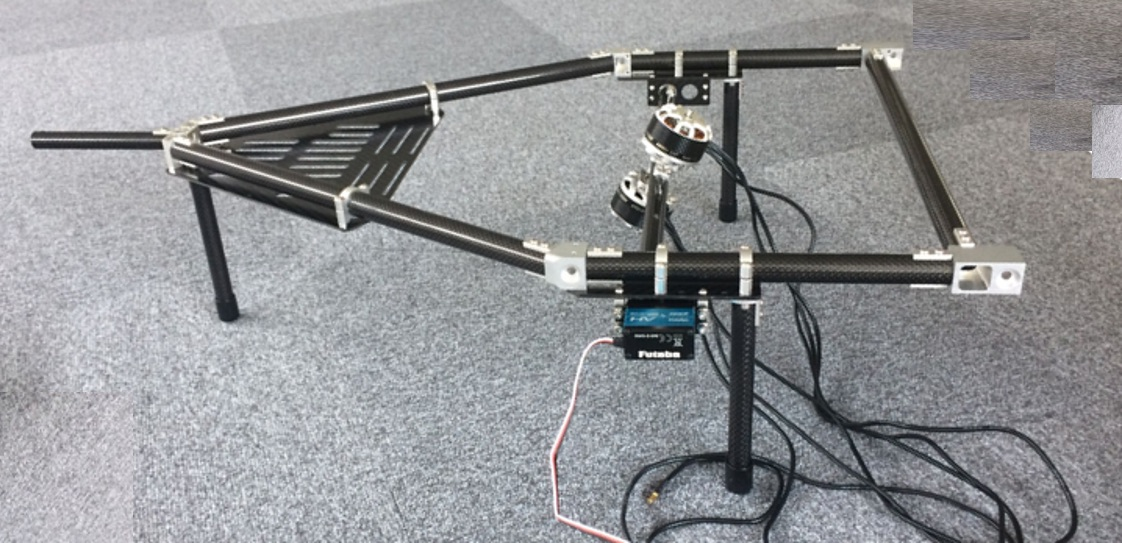
\includegraphics[clip,width=10.0cm,bb=0 0 1122 543]{./z_figure_files/chapter2/9_frame.jpeg}
		\caption{Body frame}
		\label{fig:frame}
	\end{center}
\end{figure}

\begin{figure}[h]
	\begin{center}
		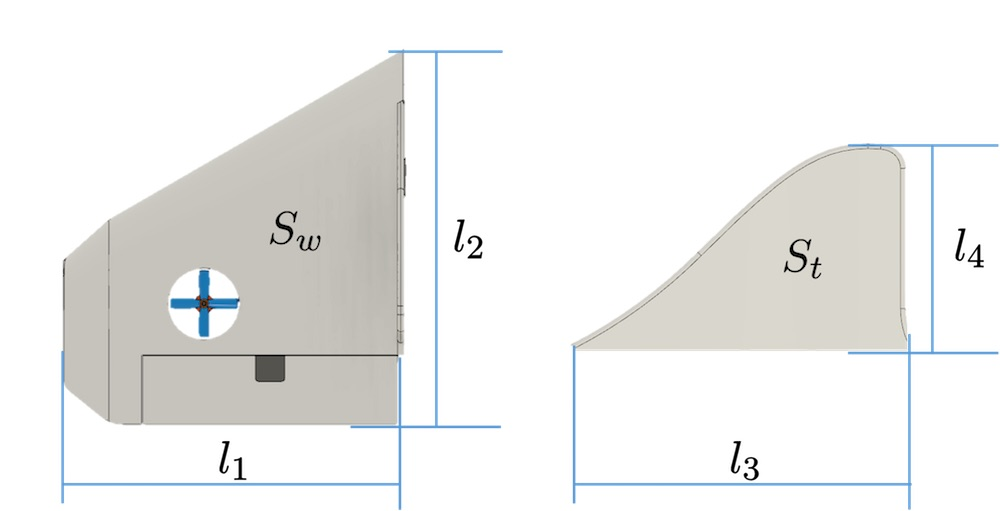
\includegraphics[clip,width = 10.0cm, bb=0 0 1000 511]{./z_figure_files/chapter2/10_Wings.jpeg}
		\caption{Main wing and vertical wing}
		\label{fig:wings}
	\end{center}
\end{figure}

\begin{table}[h]
	\begin{center}
		\caption{Specifications of the wings}
		\label{wingspec}
		\begin{tabular}{|c|c|}\hline
			Wing area($S_w$) & $0.1677\times2$[m$^2$]\\ \hline
			Wing area($S_t$) & $0.0474\times2$[m$^2$]\\ \hline
			Length($l_1$) & $0.52$[m]\\ \hline
			Length($l_2$) & $0.57$[m]\\ \hline
			Length($l_3$) & $0.36$[m]\\ \hline
			Length($l_4$) & $0.23$[m]\\ \hline
		\end{tabular}
	\end{center}
\end{table}
\begin{table}[h]
	\begin{center}
		\caption{Sensors and onboard computer}
		\label{tab:Tab2.2}
		\begin{tabular}{|c|c|} \hline
			Onboard computer & 3D Robotics Pixhawk(CPU+IO)\\ \hline
			Acceleration and magnetic filed sensor & STMicroelectoronics LSM303D\\ \hline
			Gyro sensor & STMicroelectoronics L3GD20H\\ \hline
			Barometric pressure sensor & Measurement Specialties MS5611\\ \hline
			GPS sensor & u-blox LEA-6H\\ \hline
			Airspeed senser & MS4525DO\\ \hline
		\end{tabular}
	\end{center}
\end{table}
\begin{figure}[h]
	\begin{center}
		\begin{tabular}{c}

			\begin{minipage}{0.33\hsize}
				\begin{center}
					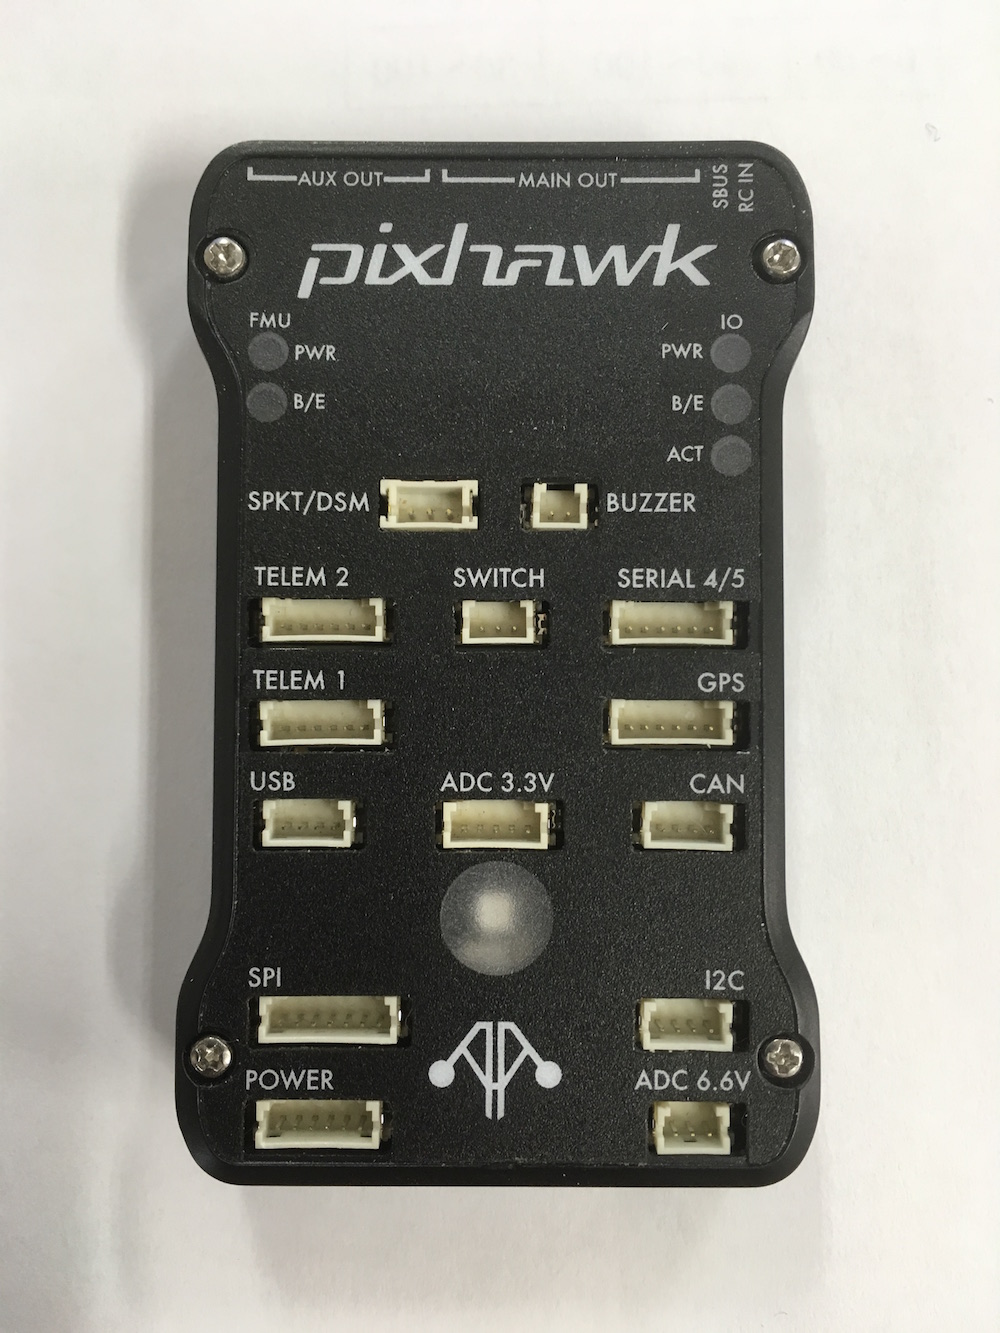
\includegraphics[clip,width=4.5cm,bb=0 0 1000 1333]{./z_figure_files/chapter2/11_pixhawk.JPG}
					\caption{Onboard computer with sensors}
					\label{fig:pixhawk}
				\end{center}
			\end{minipage}

			\begin{minipage}{0.33\hsize}
				\begin{center}
					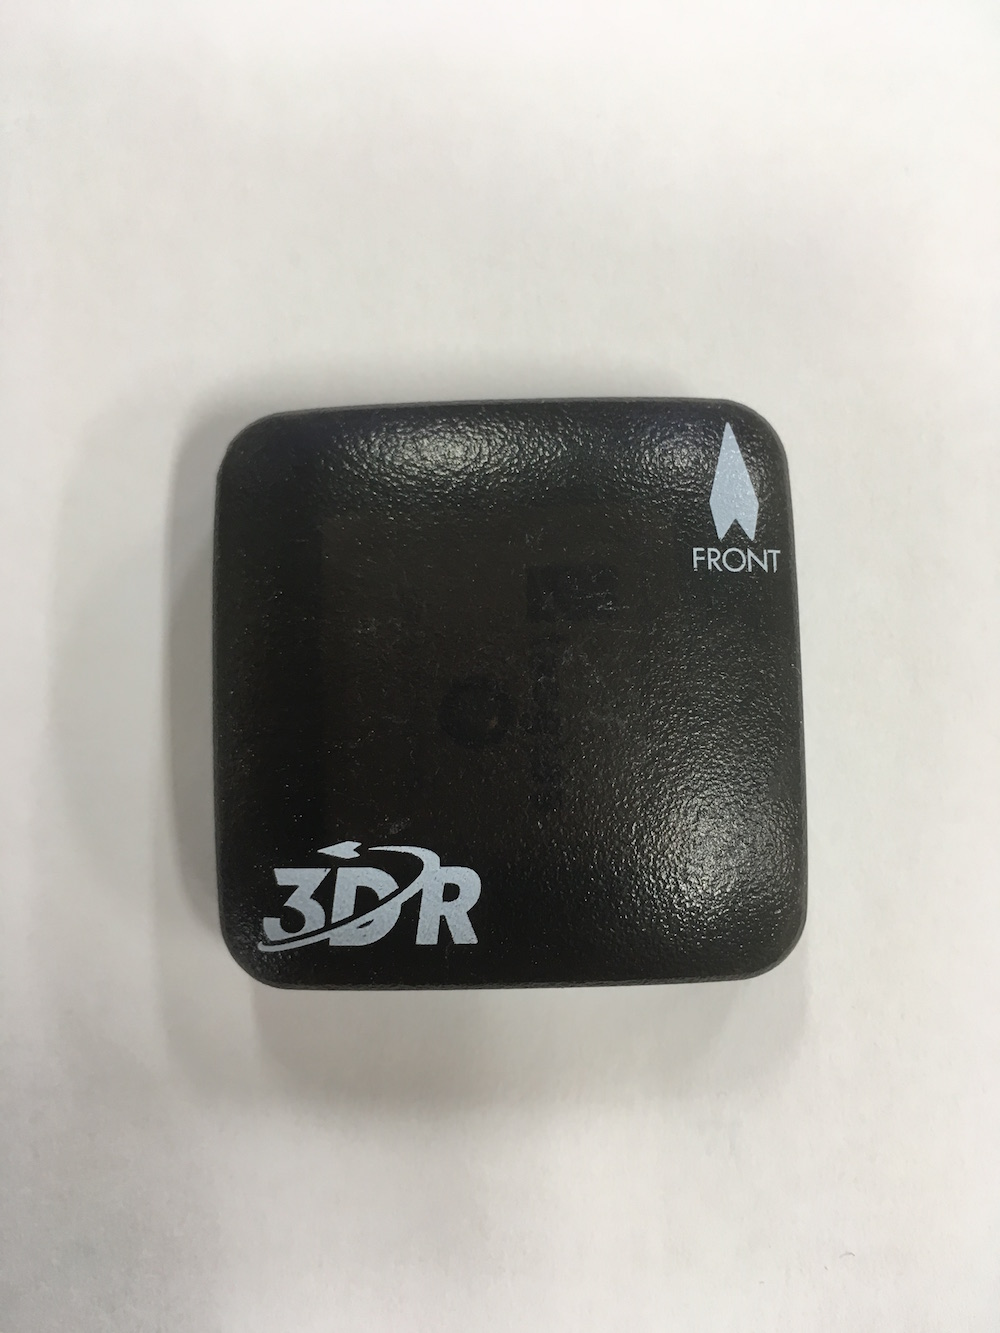
\includegraphics[clip,width=4.5cm,bb=0 0 1000 1333]{./z_figure_files/chapter2/12_GPS.JPG}
					\caption{GPS sensor}
					\label{fig:GPS}
				\end{center}
			\end{minipage}

			\begin{minipage}{0.33\hsize}
				\begin{center}
					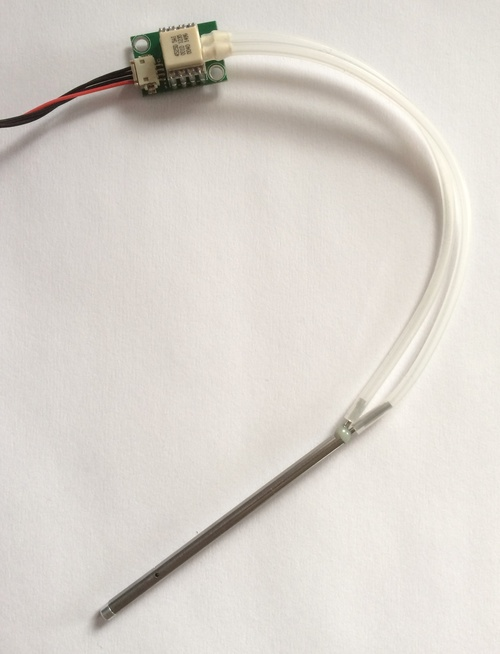
\includegraphics[clip,width=4.0cm,bb=0 0 500 654]{./z_figure_files/chapter2/13_pitot.png}
					\caption{Airspeed sensor}
					\label{fig:pitot}
				\end{center}
			\end{minipage}

		\end{tabular}
	\end{center}
\end{figure}
